%
%  untitled
%
%  Created by Parham Aram on 2010-07-14.
%  Copyright (c) 2010 . All rights reserved.
%
\documentclass[]{article}

% Setup for fullpage use
\usepackage{fullpage}

\usepackage[pdftex]{graphicx}


% More symbols
\usepackage{amsmath}
\usepackage{amssymb}

\usepackage[usenames,dvipsnames]{color}
\newcommand{\dean}[1]{\textcolor{red}{#1}}
\newcommand{\parham}[1]{\textcolor{blue}{#1}}

\begin{document}


\renewcommand{\theequation}{S1.\arabic{equation}}


\subsection*{Estimation of Connectivity Kernel Support}
The support of the connectivity kernel can be inferred using spatial correlation analysis. The method presented in this paper is based on a similar published method, where the kernel support was estimated using correlation analysis for a linear system described by an IDE~\cite{Scerri2009}. To demonstrate the method for the neural field model we assume the sensors are infinitesimally close (continuous observation). The spatial cross-correlation function between consecutive observations is defined as 
\begin{align}
	R_{y_{t},y_{t+1}}(\boldsymbol{\tau}) &= \mathbf{E}\left[ y_{t}\left(\mathbf{r}\right) y_{t+1}\left(\mathbf{r}+\boldsymbol{\tau}\right) \right] \\
	&= \mathbf{E}\left[\left(m\left(\mathbf{r}\right) \ast v_t\left(\mathbf{r}\right) + \boldsymbol{\varepsilon}_t\left(\mathbf{r}\right) \right) \times \left( m\left(\mathbf{r}+\boldsymbol{\tau}\right) \ast v_{t+1}\left(\mathbf{r}+\boldsymbol{\tau}\right) + \boldsymbol{\varepsilon}_{t+1}\left(\mathbf{r}+\boldsymbol{\tau}\right)\right) \right], \label{eq:ObsXCorr}
\end{align}
where $\mathbf{E}[\cdot]$ is the expected value. Since the observation noise is zero mean, temporally white and independent of the field, equation~\ref{eq:ObsXCorr} reduces to
\begin{equation}
	R_{y_{t},y_{t+1}}(\boldsymbol{\tau}) = \mathbf{E}\left[ m\left(\mathbf{r}\right) \ast v_t\left(\mathbf{r}\right) \times m\left(\mathbf{r}+\boldsymbol{\tau}\right) \ast v_{t+1}\left(\mathbf{r}+\boldsymbol{\tau}\right) \right].
\end{equation}
Substituting in equation~\ref{DiscreteTimeModel}  for $v_{t+1}\left(\mathbf{r}\right)$, the cross-correlation function is
\begin{align}
	R_{y_{t},y_{t+1}}(\boldsymbol{\tau}) &= \mathbf{E}\left[ m\left(\mathbf{r}\right) \ast v_t\left(\mathbf{r}\right) \times m\left(\mathbf{r}+\boldsymbol{\tau}\right) \ast \left( \xi v_t\left(\mathbf{r}+\boldsymbol{\tau}\right) + T_s w\left(\mathbf{r}+\boldsymbol{\tau}\right) \ast f\left(v_t\left(\mathbf{r}+\boldsymbol{\tau}\right)\right) + e_t\left(\mathbf{r}+\boldsymbol{\tau}\right)\right) \right] \\	
	 &= \xi \mathbf{E}\left[ m\left(\mathbf{r}\right) \ast v_t\left(\mathbf{r}\right) \times m\left(\mathbf{r}+\boldsymbol{\tau}\right) \ast v_t\left(\mathbf{r}+\boldsymbol{\tau}\right) \right] \nonumber \\
	&+ T_s\mathbf{E}\left[ m\left(\mathbf{r}\right) \ast v_t\left(\mathbf{r}\right) \times m\left(\mathbf{r}+\boldsymbol{\tau}\right) \ast w\left(\mathbf{r}+\boldsymbol{\tau}\right) \ast f\left(v_t\left(\mathbf{r}+\boldsymbol{\tau}\right)\right) \right] \nonumber \\
	&+ \mathbf{E}\left[ m\left(\mathbf{r}\right) \ast v_t\left(\mathbf{r}\right) \times m\left(\mathbf{r}+\boldsymbol{\tau}\right) \ast e_t\left(\mathbf{r}+\boldsymbol{\tau}\right) \right]
	\\
	&= R_1(\boldsymbol{\tau}) + R_2(\boldsymbol{\tau}) + R_3(\boldsymbol{\tau}).\label{eq:spatialxcorr} 
\end{align}
The first term, $R_1(\boldsymbol{\tau})$, can be simplified to
\begin{align}
	R_1(\boldsymbol{\tau}) &= \xi \mathbf{E}\left[ m\left(\mathbf{r}\right) \ast v_t\left(\mathbf{r}\right) \times m\left(\mathbf{r}+\boldsymbol{\tau}\right) \ast v_t\left(\mathbf{r}+\boldsymbol{\tau}\right) \right] \\
	&= \xi\left( R_{y_{t},y_{t}}(\boldsymbol{\tau}) - \sigma_{\varepsilon}\delta_K\left(\boldsymbol{\tau}\right) \right). \label{eq:R1}
\end{align}
The second term
\begin{equation}
	R_2(\boldsymbol{\tau}) = T_s\mathbf{E}\left[ m\left(\mathbf{r}\right) \ast v_t\left(\mathbf{r}\right) \times m\left(\mathbf{r}+\boldsymbol{\tau}\right) \ast w\left(\mathbf{r}+\boldsymbol{\tau}\right) \ast f\left(v_t\left(\mathbf{r}+\boldsymbol{\tau}\right)\right) \right]
\end{equation}
Now we assume that the sigmoid activation function, $f(\cdot)$, can be approximated by the piecewise function
\begin{equation}
	\hat{f}(v_t(\mathbf{r}')) = \left\{ \begin{array}{ll}
		0, & v_t(\mathbf{r}') \le v_1 \\
		\varsigma v_t(\mathbf{r}'), &  v_1 < v_t(\mathbf{r}') < v_2 \\
		1, & v_t(\mathbf{r}') \ge v_2 \\ 
		\end{array}\right.
\end{equation}
Furthermore, we assume the field is in the linear region of the piecewise function for the majority of the time giving
\begin{equation}
	R_2(\boldsymbol{\tau}) \approx T_s\mathbf{E}\left[ m\left(\mathbf{r}\right) \ast v_t\left(\mathbf{r}\right) \times m\left(\mathbf{r}+\boldsymbol{\tau}\right) \ast w\left(\mathbf{r}+\boldsymbol{\tau}\right) \ast \varsigma v_t\left(\mathbf{r}+\boldsymbol{\tau}\right) \right].
\end{equation}
$R_2(\boldsymbol{\tau})$ can be written as
\begin{align}
	R_2(\boldsymbol{\tau}) &\approx	T_s \varsigma \mathbf{E}\left[ \hat{y}_t\left(\mathbf{r}\right) \times \hat{y}_t\left(\mathbf{r}+\boldsymbol{\tau}\right) \ast w\left(\mathbf{r}+\boldsymbol{\tau}\right)\right] \\
	&= T_s \varsigma \mathbf{E}\left[ \hat{y}_t\left(\mathbf{r}\right)  \int_{\Omega}\hat{y}_t\left(\mathbf{r'}\right) w\left(\mathbf{r}+\boldsymbol{\tau}-\mathbf{r'}\right) d\mathbf{r'} \right] \\
	&= T_s \varsigma \mathbf{E}\left[  \int_{\Omega}\hat{y}_t\left(\mathbf{r}\right)\hat{y}_t\left(\mathbf{r'}\right) w\left(\mathbf{r}+\boldsymbol{\tau}-\mathbf{r'}\right) d\mathbf{r'} \right] \\
	&= T_s \varsigma \mathbf{E}\left[  \int_{\Omega}\hat{y}\left(\mathbf{r}\right)\hat{y}_t\left(\mathbf{r'}+\mathbf{r}\right) w\left(\boldsymbol{\tau}-\mathbf{r'}\right) d\mathbf{r'} \right] \\
	&= T_s \varsigma   \int_{\Omega}\mathbf{E}\left[\hat{y}_t\left(\mathbf{r}\right)\hat{y}_t\left(\mathbf{r'}+\mathbf{r}\right) \right] w\left(\boldsymbol{\tau}-\mathbf{r}'\right) d\mathbf{r'} \nonumber \\
	&= \frac{T_s \varsigma}{\xi} \int_{\Omega} R_1(\mathbf{r'}) w\left(\boldsymbol{\tau}-\mathbf{r}'\right) d\mathbf{r'} \nonumber \\
	&= \frac{T_s \varsigma}{\xi} \left(R_1 \ast w\right)\left(\boldsymbol{\tau}\right)\\
\end{align}
% This can be simplified to
% \begin{align}
% 	R_2(\boldsymbol{\tau}) &\approx T_s \varsigma \left( R_{y_{t},y_{t}}(\boldsymbol{\tau}) - \sigma_{\varepsilon}^2 \delta_K\left(\boldsymbol{\tau}\right) \right) \ast w\left(\boldsymbol{\tau}\right) \\
% 	&= \frac{T_s \varsigma}{\xi} R_1(\boldsymbol{\tau}) \ast w\left(\boldsymbol{\tau}\right)
% \end{align}
The last term on the right hand side of equation~\ref{eq:spatialxcorr} is
\begin{equation}
	R_3(\boldsymbol{\tau}) = 0,
\end{equation}
since the disturbance added to the field at time $t$ and assumed to be uncorrelated to the field at time $t$. Therefore 
\begin{equation}
	R_{y_{t},y_{t+1}}(\boldsymbol{\tau}) - R_1(\boldsymbol{\tau}) \approx \frac{T_s \varsigma}{\xi} \left(R_1 \ast w\right)\left(\boldsymbol{\tau}\right).
\end{equation}
Now, by taking the Fourier transform we get
\begin{equation}
	\mathcal{F}\left\{R_{y_{t},y_{t+1}}(\boldsymbol{\tau})\right\} - \mathcal{F}\left\{R_1(\boldsymbol{\tau})\right\} \approx \frac{T_s \varsigma}{\xi} \mathcal{F}\left\{R_1(\boldsymbol{\tau})\right\} \mathcal{F}\left\{ w\left(\boldsymbol{\tau}\right)\right\}.
\end{equation}
This simplifies to
\begin{equation}
	\frac{\xi}{T_s \varsigma} \left(\frac{\mathcal{F}\left\{R_{y_{t},y_{t+1}}(\boldsymbol{\tau})\right\}}{\mathcal{F}\left\{R_1(\boldsymbol{\tau})\right\}} - 1\right) \approx  \mathcal{F}\left\{ w\left(\boldsymbol{\tau}\right)\right\}.
\end{equation}
Now substituting back in equation~\ref{eq:R1}, we can write

\begin{align}
	\mathcal{F}\left\{ w\left(\boldsymbol{\tau}\right)\right\} &\approx \frac{\xi}{T_s \varsigma} \left(\frac{\mathcal{F}\left\{R_{y_{t},y_{t+1}}(\boldsymbol{\tau})\right\}}{\mathcal{F}\left\{\xi\left( R_{y_{t},y_{t}}(\boldsymbol{\tau}) - \sigma_{\varepsilon}^2\delta_K\left(\boldsymbol{\tau}\right) \right)\right\}} - 1\right)  \\
	&= \frac{1}{T_s \varsigma} \left(\frac{\mathcal{F}\left\{R_{y_{t},y_{t+1}}(\boldsymbol{\tau})\right\}}{\mathcal{F}\left\{ R_{y_{t},y_{t}}(\boldsymbol{\tau})\right\} - \sigma_{\varepsilon}^2 } - \xi\right) \\
	&= \frac{1}{T_s \varsigma} \left(\frac{S_{y_{t},y_{t+1}}\left(\boldsymbol{\nu}\right)}{S_{y_{t},y_{t}}\left(\boldsymbol{\nu}\right) - \sigma_{\varepsilon}^2 } - \xi\right)
\end{align}


 This equation states that the support of the kernel can be estimated given knowledge of $\sigma_\varepsilon^2$. Furthermore, is we assume a local coupling (at $\boldsymbol\tau=0$) regime, either excitation or inhibition, than we don't even need to know $\sigma_\varepsilon^2$. The peak in the kernel at $\mathbf{r}=0$ will be bigger or smaller if we guess incorrectly and the kernel parameters can do the rest! 
\begin{figure}[!ht]
\begin{center}
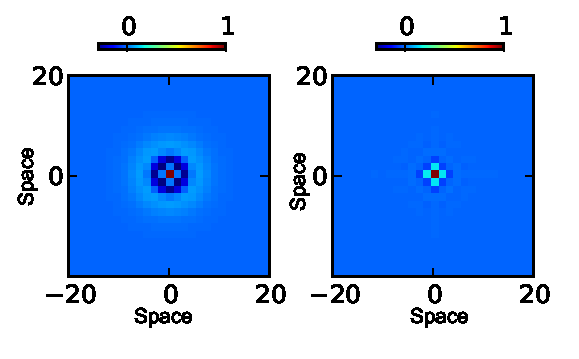
\includegraphics{./Figures/KernelWidthEstimation.pdf}
\end{center}
\caption{{\bf Estimation of Connectivity Kernel Support}. The kernel values are normalised. True  and estimated kernels are shown with solid and dotted lines respectively.}
\label{fig:KernelWidth}
\end{figure}
\newpage
\subsection*{Estimation of Disturbance Support}
\begin{align}
	R_{y_{t+1},y_{t+1}}(\boldsymbol{\tau}) &= \mathbf{E}\left[ y_{t+1}\left(\mathbf{r}\right) y_{t+1}\left(\mathbf{r}+\boldsymbol{\tau}\right) \right] \nonumber \\
	&= \mathbf{E}\left[\left(z_{t+1}\left(\mathbf r\right)  + \boldsymbol{\varepsilon}_{t+1}\left(\mathbf{r}\right) \right) \times \left(z_{t+1}\left(\mathbf{r}+\boldsymbol{\tau}\right)+ \boldsymbol{\varepsilon}_{t+1}\left(\mathbf{r}+\boldsymbol{\tau}\right)\right) \right] \nonumber \\
 &= \mathbf{E}\left[z_{t+1}\left(\mathbf r\right)  \times z_{t+1}\left(\mathbf{r}+\boldsymbol{\tau}\right) \right]+\sigma_{\epsilon}^2\delta_{K}\left(\boldsymbol\tau\right),\label{eq:ObsXCorrtplusone}
\end{align}
where
\begin{align}
z_{t+1}\left(\mathbf r\right)&=\left(m\ast v_{t+1}\right)\left(\mathbf{r}\right) \nonumber \\
&=\xi z_{t}\left(\mathbf r\right)+T_s\varsigma\left(z_t \ast w\right)\left(\mathbf r\right)+\left(m\ast e_t\right)\left(\mathbf r\right)\label{eq:zvariable}
\end{align}
substituting in equation \ref{eq:ObsXCorrtplusone} for $z_{t+1}$ we have
\begin{align}
	R_{y_{t+1},y_{t+1}}(\boldsymbol{\tau}) &=  \xi^2\mathbf{E}\left[ z_t\left(\mathbf r\right)z_t\left(\mathbf r+\boldsymbol \tau\right)\right] \nonumber \\
						&+\xi T_s\varsigma \ \mathbf{E}\left[z_t\left(\mathbf r\right)\left(z_t \ast w\right)\left(\mathbf r+\boldsymbol\tau\right)\right]\nonumber \\
						&+\xi T_s\varsigma \ \mathbf{E}\left[\left(z_t \ast w\right)\left(\mathbf r\right)z_t\left(\mathbf r+\boldsymbol\tau\right)\right]\nonumber \\
						&+T_s^2\varsigma^2 \ \mathbf{E}\left[\left(z_t \ast w\right)\left(\mathbf r\right)\left(z_t \ast w\right)\left(\mathbf r+\boldsymbol\tau\right)\right]\nonumber \\
						&+\mathbf{E}\left[\left(m \ast e_t\right)\left(\mathbf r\right)\left(m \ast e_t\right)\left(\mathbf r+\boldsymbol\tau\right)\right]+\sigma_{\epsilon}^2\delta_{K}\left(\boldsymbol\tau\right)\label{eq:AutocorrExpansion}
\end{align}
Equation \ref{eq:AutocorrExpansion} can be written in terms of $R_1\left(\boldsymbol\tau\right)$ and $R_2\left(\boldsymbol\tau\right)$ as
\begin{align}
R_{y_{t+1},y_{t+1}}(\boldsymbol{\tau}) &=\xi \left(R_1\left(\boldsymbol\tau\right)+ R_2\left(\boldsymbol\tau\right)+R_2\left(\boldsymbol-\tau\right)\right) \nonumber \\
&+\xi T_s \varsigma\left(w\ast R_2\right)\left(\boldsymbol\tau\right)+\left(m\ast m \ast \gamma\right)\left(\boldsymbol\tau\right)+\sigma_{\epsilon}^2\delta_{K}\left(\boldsymbol\tau\right)\label{eq:AutocorrIntermsofR}
\end{align}
Equation \ref{eq:AutocorrIntermsofR} is correct for all times, noting $R_{y_{t},y_{t+1}}(\boldsymbol{\tau})=R_1\left(\boldsymbol\tau\right)+ R_2\left(\boldsymbol\tau\right) $ therefore we cam wite
\begin{align}
R_{y_{t},y_{t}}(\boldsymbol{\tau}) &=\xi \left(R_{y_{t},y_{t+1}}(\boldsymbol{\tau})+R_2\left(\boldsymbol-\tau\right)\right) \nonumber \\
&+\xi T_s \varsigma\left(w\ast R_2\right)\left(\boldsymbol\tau\right)+\left(m\ast m \ast \gamma\right)\left(\boldsymbol\tau\right)+\sigma_{\epsilon}^2\delta_{K}\left(\boldsymbol\tau\right)
\end{align}
taking Fourier transform we have
\begin{align}
 \mathcal{F}\left\{\left(m\ast m\ast \gamma\right)\left(\boldsymbol\tau\right)\right\}&=S_{y_{t},y_{t}}\left(\boldsymbol\nu\right)-\xi S_{y_{t},y_{t+1}}\left(\boldsymbol\nu\right)-\xi \mathcal{F}\left\{R_2\left(-\boldsymbol\tau\right)\right\} \nonumber\\
&-\xi T_s \varsigma  \mathcal{F}\left\{w\left(\boldsymbol\tau\right)\right\}\mathcal{F}\left\{R_2\left(\boldsymbol\tau\right)\right\}-\sigma_{\epsilon}^2 \label{eq:SensorsConvgamma}
\end{align}
where
\begin{align}
 \mathcal{F}\left\{R_2\left(\boldsymbol\tau\right)\right\}=S_{y_{t},y_{t+1}}\left(\boldsymbol\nu\right)-\xi \left(S_{y_{t},y_{t}}\left(\boldsymbol\nu\right)-\sigma_{\epsilon}^2\right)
\end{align}
and
\begin{align}
 \mathcal{F}\left\{w\left(\boldsymbol\tau\right)\right\}\mathcal{F}\left\{R_2\left(\boldsymbol\tau\right)\right\}&=\frac{1}{T_s \varsigma}\left[\frac{S_{y_{t},y_{t+1}}^2\left(\boldsymbol\nu\right)}{S_{y_{t},y_{t}}\left(\boldsymbol\nu\right)-\sigma_{\epsilon}^2}-2\xi S_{y_{t},y_{t+1}}\left(\boldsymbol\nu\right)+\xi^2\left(S_{y_{t},y_{t}}\left(\boldsymbol\nu\right)-\sigma_{\epsilon}^2\right)\right]
\end{align}
and therefore equation \ref{eq:SensorsConvgamma} can be written as 
\begin{align}
 \mathcal{F}\left\{\left(m\ast m\ast \gamma\right)\left(\boldsymbol\tau\right)\right\}&=S_{y_{t},y_{t}}\left(\boldsymbol\nu\right)-\xi S_{y_{t},y_{t+1}}\left(\boldsymbol\nu\right) \nonumber \\
&-\xi S_{y_{t},y_{t+1}}\left(-\boldsymbol\nu\right)-\xi^2 \left(S_{y_{t},y_{t}}\left(\boldsymbol\nu\right)-\sigma_{\epsilon}^2\right) \nonumber\\
&-\xi  \left[\frac{S_{y_{t},y_{t+1}}^2\left(\boldsymbol\nu\right)}{S_{y_{t},y_{t}}\left(\boldsymbol\nu\right)-\sigma_{\epsilon}^2}-2\xi S_{y_{t},y_{t+1}}\left(\boldsymbol\nu\right)+\xi^2\left(S_{y_{t},y_{t}}\left(\boldsymbol\nu\right)-\sigma_{\epsilon}^2\right)\right]-\sigma_{\epsilon}^2
\end{align}
\begin{figure}[!ht]
\begin{center}
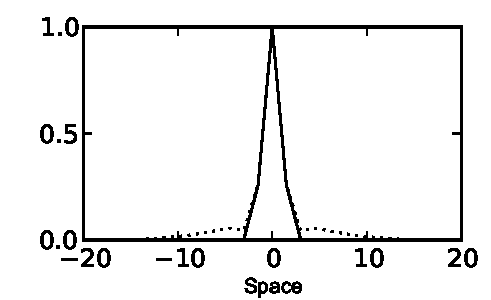
\includegraphics{./Figures/DisturbanceWidthEstimation.pdf}
\end{center}
\caption{{\bf Estimation of $\left(m\ast m \ast \gamma \right)\left(\boldsymbol \tau\right) $ width}. Values are normalised. True  and estimated values are shown with solid and dotted lines respectively.}
\label{fig:DisturbanceWidth}
\end{figure}

% Putting to other two terms back together we can write
% \begin{equation}
% 	R_{y_{t},y_{t+1}}(\boldsymbol{\tau}) = \mathbf{E}\left[ m\left(\mathbf{r}\right) \ast v_t\left(\mathbf{r}\right) \times m\left(\mathbf{r}+\boldsymbol{\tau}\right) \ast \left(\xi v_t\left(\mathbf{r}+\boldsymbol{\tau}\right) + T_s w\left(\mathbf{r}+\boldsymbol{\tau}\right) \ast f\left(v_t\left(\mathbf{r}+\boldsymbol{\tau}\right)\right) \right) \right]
% \end{equation}
% Now we assume that the sigmoid activation function, $f(\cdot)$, can be approximated by the piecewise function
% \begin{equation}
% 	\hat{f}(v_t(\mathbf{r}')) = \left\{ \begin{array}{ll}
% 		0, & v_t(\mathbf{r}') \le v_1 \\
% 		\varsigma v_t(\mathbf{r}'), &  v_1 < v_t(\mathbf{r}') < v_2 \\
% 		1, & v_t(\mathbf{r}') \ge v_2 \\ 
% 		\end{array}\right.
% \end{equation}
% Furthermore, we assume the field is in the linear region of the piecewise function for the majority of the time. 
% \begin{equation}
% 	R_{y_{t},y_{t+1}}(\boldsymbol{\tau}) \approx \mathbf{E}\left[ m\left(\mathbf{r}\right) \ast v_t\left(\mathbf{r}\right) \times m\left(\mathbf{r}+\boldsymbol{\tau}\right) \ast \left(\xi v_t\left(\mathbf{r}+\boldsymbol{\tau}\right) + T_s w\left(\mathbf{r}+\boldsymbol{\tau}\right) \ast \varsigma v_t\left(\mathbf{r}+\boldsymbol{\tau}\right) \right) \right]
% \end{equation}
% Now we take the Fourier transform of the terms inside the expectation giving
% \begin{align}
% 	R_{y_{t},y_{t+1}}(\boldsymbol{\tau}) &\approx \mathbf{E}\left[\mathcal{F}^{-1} \left\{M(\boldsymbol{\nu})V(\boldsymbol{\nu}) \ast \left(\xi e^{i\boldsymbol{\nu}^{\top}\boldsymbol{\tau}} M(\boldsymbol{\nu}) e^{i\boldsymbol{\nu}^{\top}\boldsymbol{\tau}} V(\boldsymbol{\nu}) + T_s e^{i\boldsymbol{\nu}^{\top}\boldsymbol{\tau}} M(\boldsymbol{\nu}) e^{i\boldsymbol{\nu}^{\top}\boldsymbol{\tau}} W(\boldsymbol{\nu}) e^{i\boldsymbol{\nu}^{\top}\boldsymbol{\tau}} \varsigma V(\boldsymbol{\nu}) \right) \right\} \right] \\
% 	&= \mathbf{E}\left[\mathcal{F}^{-1} \left\{M(\boldsymbol{\nu}) V(\boldsymbol{\nu}) \ast \left(\xi e^{2i\boldsymbol{\nu}^{\top}\boldsymbol{\tau}} M(\boldsymbol{\nu}) V(\boldsymbol{\nu}) + T_s \varsigma e^{2i\boldsymbol{\nu}^{\top}\boldsymbol{\tau}} M(\boldsymbol{\nu})  V(\boldsymbol{\nu}) e^{i\boldsymbol{\nu}^{\top}\boldsymbol{\tau}} W(\boldsymbol{\nu}) \right) \right\} \right]
% \end{align}
% Expand brackets
% \begin{equation}
% 	R_{y_{t},y_{t+1}}(\boldsymbol{\tau}) \approx \mathbf{E}\left[\mathcal{F}^{-1} \left\{M(\boldsymbol{\nu}) V(\boldsymbol{\nu}) \ast  \xi e^{2i\boldsymbol{\nu}^{\top}\boldsymbol{\tau}} M(\boldsymbol{\nu}) V(\boldsymbol{\nu}) + M(\boldsymbol{\nu}) V(\boldsymbol{\nu}) \ast T_s \varsigma e^{2i\boldsymbol{\nu}^{\top}\boldsymbol{\tau}} M(\boldsymbol{\nu}) V(\boldsymbol{\nu}) e^{i\boldsymbol{\nu}^{\top}\boldsymbol{\tau}} W(\boldsymbol{\nu}) \right\} \right]
% \end{equation}
% 
% Now taking the inverse Fourier transform we get
% \begin{equation}
% 	R_{y_{t},y_{t+1}}(\boldsymbol{\tau}) \approx \mathbf{E}\left[m(\mathbf{r}) \ast v_t(\mathbf{r}) \times \xi m(\mathbf{r}+\boldsymbol{\tau}) \ast v_t(\mathbf{r}+\boldsymbol{\tau}) +  m(\mathbf{r}) \ast v_t(\mathbf{r}) \times T_s \varsigma m(\mathbf{r}+\boldsymbol{\tau}) \ast v_t(\mathbf{r}+\boldsymbol{\tau}) \ast w(\mathbf{r}+\boldsymbol{\tau}) \right]
% \end{equation}
% Split the expectation at the plus sign
% \begin{align}
% 	R_{y_{t},y_{t+1}}(\boldsymbol{\tau}) &\approx \xi \mathbf{E}\left[m(\mathbf{r}) \ast v_t(\mathbf{r}) \times  m(\mathbf{r}+\boldsymbol{\tau}) \ast v_t(\mathbf{r}+\boldsymbol{\tau}) \right] \\
% 	&+ T_s \varsigma \mathbf{E}\left[  m(\mathbf{r}) \ast v_t(\mathbf{r}) \times  m(\mathbf{r}+\boldsymbol{\tau}) \ast v_t(\mathbf{r}+\boldsymbol{\tau}) \ast w(\mathbf{r}+\boldsymbol{\tau}) \right] \\
% 	&= \xi \left(R_{y_{t},y_{t}}(\boldsymbol{\tau}) - \sigma_{\varepsilon}\delta_K\left(\boldsymbol{\tau}\right)\right) \\
% 	&+ T_s \varsigma \mathbf{E}\left[  m(\mathbf{r}) \ast v_t(\mathbf{r}) \times  m(\mathbf{r}+\boldsymbol{\tau}) \ast v_t(\mathbf{r}+\boldsymbol{\tau}) \right]  \ast w(\boldsymbol{\tau}) \\
% 	&= \xi \left( R_{y_{t},y_{t}}(\boldsymbol{\tau}) - \sigma_{\varepsilon}\delta_K\left(\boldsymbol{\tau}\right) \right) \\
% 	&+ T_s \varsigma \left( R_{y_{t},y_{t}}(\boldsymbol{\tau}) - \sigma_{\varepsilon}\delta_K\left(\boldsymbol{\tau}\right) \right) \ast w(\boldsymbol{\tau})
% \end{align}
% 
% Now rearrange to get
% \begin{align}
% 	R_{y_{t},y_{t+1}}(\boldsymbol{\tau}) - \xi \left( R_{y_{t},y_{t}}(\boldsymbol{\tau}) - \sigma_{\varepsilon}\delta_K\left(\boldsymbol{\tau}\right) \right) \approx T_s \varsigma \left( R_{y_{t},y_{t}}(\boldsymbol{\tau}) - \sigma_{\varepsilon}\delta_K\left(\boldsymbol{\tau}\right) \right) \ast w(\boldsymbol{\tau})
% \end{align}
% 
% Taking the Fourier transform gives
% \begin{equation}
% 	\frac{1}{T_s \varsigma}\mathcal{F}^{-1}\left\{\frac{\mathcal{F}\left\{ R_{y_{t},y_{t+1}}(\boldsymbol{\tau}) - \xi \left( R_{y_{t},y_{t}}(\boldsymbol{\tau}) - \sigma^2_{\varepsilon}\delta_K\left(\boldsymbol{\tau}\right) \right) \right\}} {  \mathcal{F} \left\{  R_{y_{t},y_{t}}(\boldsymbol{\tau}) - \sigma^2_{\varepsilon}\delta_K\left(\boldsymbol{\tau}\right) \right\}}\right\} \approx  w(\boldsymbol{\tau})	
% \end{equation}
% Simplify
% \begin{equation}
% 	\frac{1}{T_s \varsigma}\mathcal{F}^{-1}\left\{\frac{(1 - \xi)\mathcal{F}\left\{ R_{y_{t},y_{t+1}}(\boldsymbol{\tau}) \right\} - \xi \sigma^2_{\varepsilon} } {  \mathcal{F} \left\{  R_{y_{t},y_{t}}(\boldsymbol{\tau}) \right\} - \sigma^2_{\varepsilon} }\right\} \approx  w(\boldsymbol{\tau})	
% \end{equation}
% 
% \begin{align}
% 	R_{y_{t},y_{t+1}}(\boldsymbol{\tau}) &\approx \mathbf{E}\left[m(\mathbf{r}) \ast v_t(\mathbf{r}) \times \left( m(\mathbf{r}+\boldsymbol{\tau}) \ast v_t(\mathbf{r}+\boldsymbol{\tau}) \ast \xi\delta_D(\mathbf{r}) + T_s \varsigma m(\mathbf{r}+\boldsymbol{\tau}) \ast v_t(\mathbf{r}+\boldsymbol{\tau}) \ast  w(\mathbf{r}+\boldsymbol{\tau})\right) \right] \\
% 	&= \mathbf{E}\left[m(\mathbf{r}) \ast v_t(\mathbf{r}) \times \left( m(\mathbf{r}+\boldsymbol{\tau}) \ast \xi v_t(\mathbf{r}+\boldsymbol{\tau}) + T_s \varsigma m(\mathbf{r}+\boldsymbol{\tau}) \ast v_t(\mathbf{r}+\boldsymbol{\tau}) \ast  w(\mathbf{r}+\boldsymbol{\tau})\right) \right] \\
% 	&= \mathbf{E}\left[m(\mathbf{r}) \ast v_t(\mathbf{r}) \times  m(\mathbf{r}+\boldsymbol{\tau}) \ast \xi v_t(\mathbf{r}+\boldsymbol{\tau}) + m(\mathbf{r}) \ast v_t(\mathbf{r}) \times T_s \varsigma m(\mathbf{r}+\boldsymbol{\tau}) \ast v_t(\mathbf{r}+\boldsymbol{\tau}) \ast  w(\mathbf{r}+\boldsymbol{\tau}) \right] \\
% 	&= \mathbf{E}\left[m(\mathbf{r}) \ast v_t(\mathbf{r}) \times  m(\mathbf{r}+\boldsymbol{\tau}) \ast \xi v_t(\mathbf{r}+\boldsymbol{\tau}) \right] + \mathbf{E}\left[ m(\mathbf{r}) \ast v_t(\mathbf{r}) \times T_s \varsigma m(\mathbf{r}+\boldsymbol{\tau}) \ast v_t(\mathbf{r}+\boldsymbol{\tau}) \ast  w(\mathbf{r}+\boldsymbol{\tau}) \right] \\
% 	&= R_{y_{t},y_{t}}(\boldsymbol{\tau}) - \sigma_{\varepsilon}\delta_K\left(\boldsymbol{\tau}\right) + \mathbf{E}\left[ m(\mathbf{r}) \ast v_t(\mathbf{r}) \times T_s \varsigma m(\mathbf{r}+\boldsymbol{\tau}) \ast v_t(\mathbf{r}+\boldsymbol{\tau}) \ast  w(\mathbf{r}+\boldsymbol{\tau}) \right] \\
% 	&= R_{y_{t},y_{t}}(\boldsymbol{\tau}) - \sigma_{\varepsilon}\delta_K\left(\boldsymbol{\tau}\right) + \mathbf{E}\left[ m(\mathbf{r}) \ast v_t(\mathbf{r}) \times  m(\mathbf{r}+\boldsymbol{\tau}) \ast v_t(\mathbf{r}+\boldsymbol{\tau})\right] \ast T_s \varsigma w(\boldsymbol{\tau}) \\
% 	% 	&\parham{= \mathbf{E}\left[m(\mathbf{r}) \ast v_t(\mathbf{r}) \times m(\mathbf{r}+\boldsymbol{\tau}) \ast v_t(\mathbf{r}+\boldsymbol{\tau}) \right] \ast \mathbf{E}\left[\left( \xi\delta_D(\mathbf{r}) + T_s \varsigma w(\mathbf{r}+\boldsymbol{\tau}) \right) \right]} \label{eq:xcorr_pre_sub}
% \end{align}
% \parham{From (S1.14) to (S1.15) doesn't hold.} where $\mathcal{F}^{-1}$ denotes the inverse Fourier transform and $R_{y_{t},y_{t}}(\boldsymbol{\tau})$ is the auto-correlation of the observations, $\delta_K(\cdot)$ is the Kronecker delta function, and $\delta_D(\cdot)$ is the Dirac delta function. We define the auto-correlation of the observations as
% \begin{align}
% 	R_{y_{t},y_{t}}(\boldsymbol{\tau}) &= \mathbf{E}\left[ y_{t}\left(\mathbf{r}\right) y_{t}\left(\mathbf{r}+\boldsymbol{\tau}\right) \right]\\
% 	&= \mathbf{E}\left[m(\mathbf{r}) \ast v_t(\mathbf{r}) \times m(\mathbf{r}+\boldsymbol{\tau}) \ast v_t(\mathbf{r}+\boldsymbol{\tau})\right] + \delta_K(\boldsymbol{\tau})\sigma_{\varepsilon}^2
% \end{align}
% Rearrange to get
% \begin{equation}\label{eq:autocorr_for_sub}
% 	R_{y_{t},y_{t}}(\boldsymbol{\tau}) - \delta_K(\boldsymbol{\tau})\sigma_{\varepsilon}^2 = \mathbf{E}\left[m(\mathbf{r}) \ast v_t(\mathbf{r}) \times m(\mathbf{r}+\boldsymbol{\tau}) \ast v_t(\mathbf{r}+\boldsymbol{\tau})\right].
% \end{equation}
% Now to isolate the kernel equation~\ref{eq:autocorr_for_sub} is substituted into equation~\ref{eq:xcorr_pre_sub} and the Fourier transform is taken giving
% \begin{align}
% 	\mathcal{F}\left\{R_{y_{t},y_{t+1}}(\boldsymbol{\tau})\right\} &\approx \mathcal{F}\left\{ \left(R_{y_t,y_t}(\boldsymbol{\tau}) - \delta_K\left(\boldsymbol{\tau}\right)\sigma_{\varepsilon}^2\right) \ast \mathbf{E} \left[ \xi\delta_D(\mathbf{r})  + T_s \varsigma w(\mathbf{r}+\boldsymbol{\tau}) \right] \right\} \\
% 	&= \mathcal{F}\left\{ R_{y_t,y_t}(\boldsymbol{\tau}) - \delta_K\left(\boldsymbol{\tau}\right) \sigma_{\varepsilon}^2 \right\} \mathcal{F}\left\{\mathbf{E}[ \xi \delta_D(\mathbf{r})  + T_s \varsigma w(\mathbf{r}+\boldsymbol{\tau}) ]\right\}.
% \end{align}
% Now rearranging
% \begin{equation}
% 	\frac{\mathcal{F}\left\{R_{y_{t},y_{t+1}}(\boldsymbol{\tau})\right\}}{\mathcal{F}\left\{ R_{y_t,y_t}(\boldsymbol{\tau}) - \delta_K\left(\boldsymbol{\tau}\right)\sigma_{\varepsilon}^2 \right\}} \approx \mathcal{F}\left\{ \mathbf{E}\left[ \xi\delta_D\left(\mathbf{r}\right)  + T_s \varsigma w(\mathbf{r}+\boldsymbol{\tau}) \right]\right\}.
% \end{equation}
% Take inverse Fourier transform and rearrange to get an approximation of the kernel
% \begin{equation}
% 	\mathcal{F}^{-1}\left\{\frac{\mathcal{F}\left\{R_{y_{t},y_{t+1}}(\boldsymbol{\tau})\right\}}{\mathcal{F}\left\{ R_{y_t,y_t}(\boldsymbol{\tau}) - \delta_K\left(\boldsymbol{\tau}\right)\sigma_{\varepsilon}^2 \right\}}\right\} \approx \mathbf{E}[\xi\delta_D\left(\mathbf{r}\right)  + T_s \varsigma w(\mathbf{r}+\boldsymbol{\tau})].
% \end{equation}

\bibliographystyle{plain}
\bibliography{}
\end{document}
